\documentclass[12pt]{article}

\usepackage[top=1in,bottom=1in,left=1in,right=1in]{geometry}
\usepackage{amsmath,amssymb,mathtools}
\usepackage{xcolor}
\usepackage{graphicx}
\usepackage{hyperref}

\hypersetup{
    pdfauthor={},
    pdftitle={MATH 1075 - Lesson 6.1 Recitation}
}

\begin{document}

\vspace*{0.5in}

\begin{center}
    {\LARGE MATH 1075 - Section 7.6 Worksheet}

    \vspace{2em}

    {\large 09/24/2026}
\end{center}

\begin{figure}[htbp]
    \centering
    % Replace "my_image" with your actual file name (without extension)
    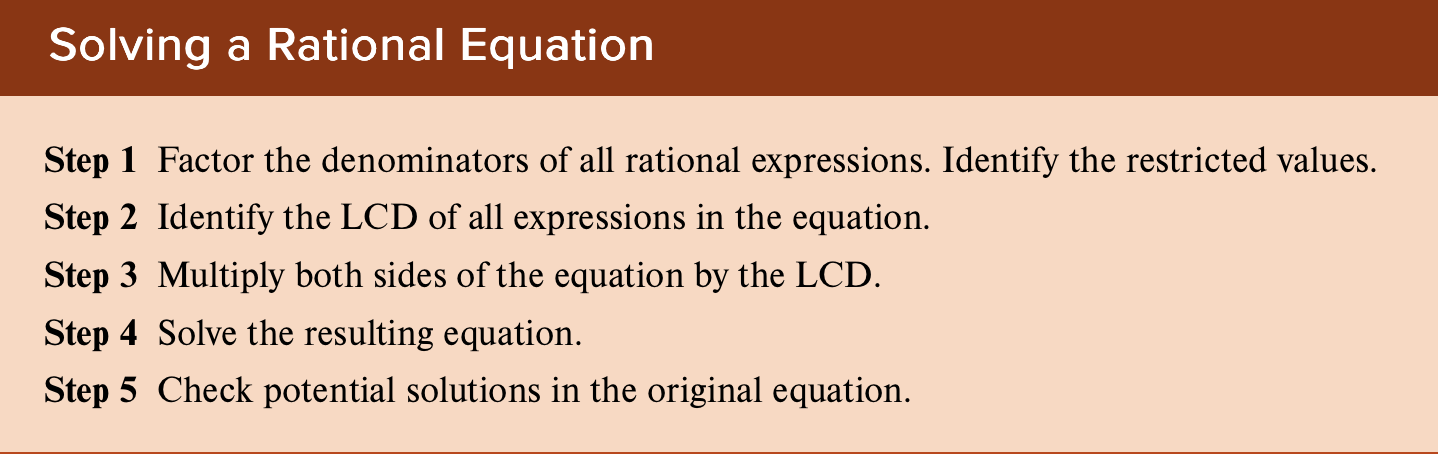
\includegraphics[width=0.9\linewidth]{Solving Rational Equation.png} 
    \label{fig:my_figure}
\end{figure}
Solve following rational equations
\vspace{1.5em}

1. $\frac{x}{2}+\frac{1}{3}=2  $

\vspace{4.5em}

2. $\frac{2}{7}-\frac{1}{x}=\frac{2}{3}     $

\vspace{4.5em}

3. $\frac{2}{x+2}=\frac{5}{3x}   $

\vspace{4.5em}

4. $\frac{t}{12}+\frac{t+3}{3t}=\frac{1}{t}      $

\vspace{4.5em}

5. $\frac{x}{x+1}-2=\frac{-1}{x+1}   $

\newpage



6. $\frac{4x}{x+3}-\frac{12}{x-3}=\frac{4x^{2}+36}{x^{2}-9}   $

\vspace{4.5em}

7. $\frac{6}{5a+10}-\frac{1}{a-5}=\frac{4}{a^{2}-3a-10}    $




\end{document}
